\section {Experimental Setup}
The setup is illustrated in Figure \ref{figExperimentalSetup}.
\begin{figure}[htbp]
    \centering
    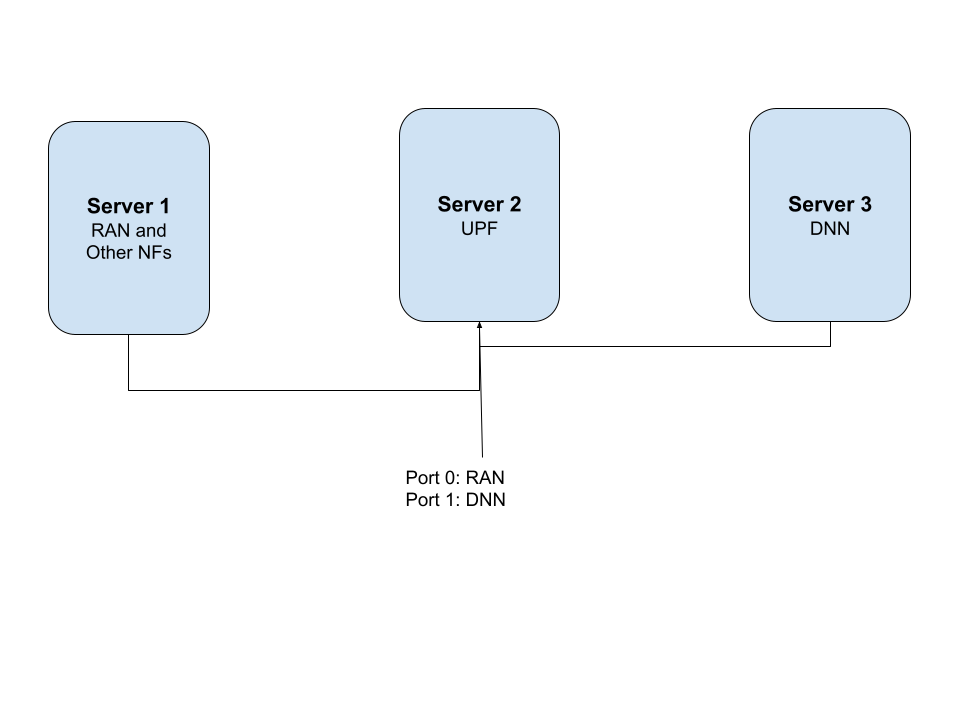
\includegraphics[width=0.7\textwidth, keepaspectratio]{./fig/Results/Setup.png}
    \caption{Experimental Setup}
    \label{figExperimentalSetup}
\end{figure}
 The main features of the setup are: 
 \begin{itemize} 
        \item \textbf{Server's Layout}
        \begin{enumerate}
                \item \textbf{Server 1} The radio access network (RAN) and other network functions responsible for authentication,
         session establishment, charging functions are simulated on server 1.  The user equipments are also 
         simulated on the same machine. The load generation in the uplink direction is the main function of this server in the data forwarding plane.
                \item \textbf{Server 2} This server hosts the user plane function (UPF). The UPF architecture is discussed 
         in detail in Chapter \ref{chapterUpfArchitecture}. Two ports on this server are used to communicate with RAN 
         (server 1) and data network name (server 3).
                 \item \textbf{Server 3} This server simulates the data network name (DNN) network function. This network 
        function is the gateway to public Internet for 5G telecommunication. This server is used to generate downlink traffic. This server is also used to mirror packets received from uplink and forwarded back in the downlinj direction. The mirroring of latency packets help in measuring end-to-end latency (Round Trip Time) at the RAN. 
        \end{enumerate} 
        \item \textbf{Hardware Configuration} 
        \begin{enumerate}
                \item \textbf{CPU} Intel Xeon Core i5 @2.20GHz. 12 cores on every NUMA node. Only a single NUMA node is used in the experiments. Hyperthreading is kept off to facilitate repeatability of results.
                \item \textbf{Memory} 8192 superpages of size 2MB are reserved initially for the whole run. The use of superpages reduces the number of TLB misses. Fragmentation due to large page sizes is dealt by DPDK libraries (see \cite{memblogdpdk}) internally while allocating memory buffers storing the incoming packets.
                \item \textbf{Cache} 32 KB L1i-cache, 32 KB L1d-cache, 256 KB L2 cache per core. 30 MB L3 cache per NUMA node. 
                \item \textbf{NIC} Intel XL710 NIC controller wih QSFP+ cables that  can handle upto 40 Gbps traffic.
        \end{enumerate}
        
\end{itemize}

\section{Experiments \label{sectionExperiments}}
After deploying Dynamic Device Personalization feature (discussed in Chapter \ref{chapterRSS}) in the RTC model, the pipeline and RTC models were compared on the parameters described in the section \ref{RTCpipelineComparison}. The main questions addressed are 
\begin{enumerate}
        \item  How does the transmit throughput for a single core vary with \textbf{increasing packet sizes} in both uplink and downlink directions? 
        \item  How does the transmit throughput for a single core vary with the increase in \textbf{number of active UEs/sessions} ? 
        \item How does throughput scale with the \textbf{number of cores}? 
        \item \textbf{Skewed Traffic} How do Pipeline and RTC handle skewed traffic with a few UEs as heavy hitters?
       \item \textbf{Dynamic Balancing} What is the impact on latency and packet drop rate  or throughput during the transient phase of
        dynamic increase in number of worker cores to handle the increasing traffic? 
\end{enumerate}
\subsection{Throughput v/s. Payload Size \label{subSectiontptPayload}}
A single core is active in both uplink and downlink directions to handle incoming
 traffic. The load generated at RAN/DNN is more than
 what a single core can handle and the actual transmit throughput is measured. 

It is expected that the number of packets processed per second should remain
constant irrespective of packet size as header processing is the main task and
size of the header is independent of packet size.
\begin{figure}[htbp]
    \centering
    \subfigure[]{
    \fbox{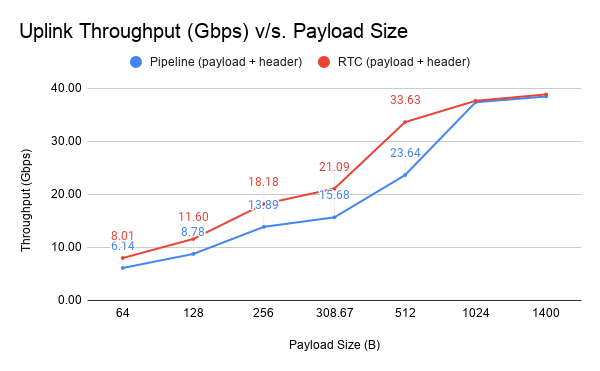
\includegraphics[width=70mm,height=50mm]{./fig/Results/tptv_spayload/ULG.png}}
    \label{figpayloadULG}
    }
    \subfigure[]{
    \fbox{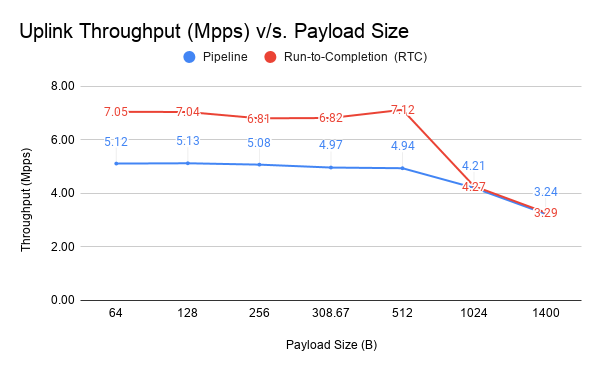
\includegraphics[width=70mm,height=50mm]{./fig/Results/tptv_spayload/ULM.png}}
    \label{figpayloadULM}
    }
    \subfigure[]{
    \fbox{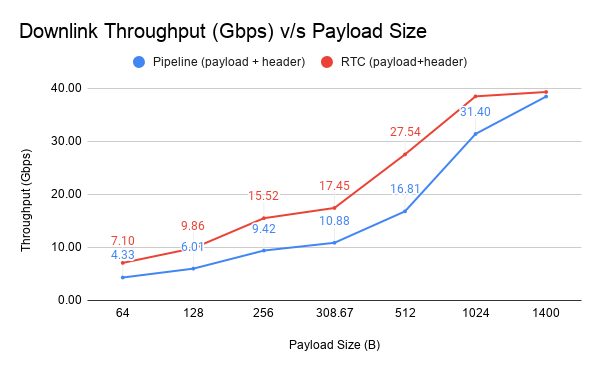
\includegraphics[width=70mm,height=50mm]{./fig/Results/tptv_spayload/DLG.png}}
    \label{figpayloadDLG}
    }
    \subfigure[]{
    \fbox{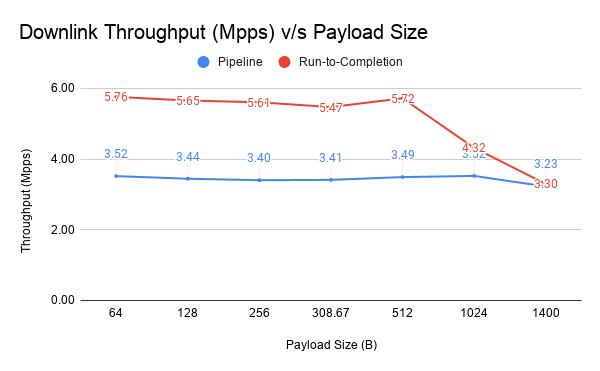
\includegraphics[width=71mm,height=50mm]{./fig/Results/tptv_spayload/DLM.png}}
    \label{figpayloadDLM}
    }
    \caption{ Throughput v/s Payload Size. Throughput calculation in Gbps includes header size.}
        \label{figurepayload}
    \end{figure}


\subsubsection{Results}
Figure \ref{figurepayload} shows the results. The measurements are made in both uplink and
downlink direction for different payload sizes. Each run is of the duration of 150
 seconds. The number of sessions maintained in the UPF is equal to 100000. A total
of 65536 UEs are kept active while making measurements. It was observed that
there was negligible variation in the packets processed per second when readings
were taken every second. The main results are
\begin{itemize}
        \item Packets processed per second is independent of the packet size. The packets
        processed per second for 1024 Byte packet decreases due to the saturation of link/NIC.  
        \item RTC gives 30-40\% higher throughput than pipeline for different payload sizes as expected (see also section \ref{RTCpipelineComparison}).
        \item Uplink performance is better than downlink performance. This is because of
        \textbf{GTP encapsulation overhead} in downlink direction.
 \end{itemize}

\subsection{Throughput v/s. Number of active sessions/UEs}
The experiment with same conditions as section \ref{subSectiontptPayload} was conducted. However the payload size is kept fixed  at 64 Bytes and the number of active UEs are varied.
Performance degradation  is expected with the increasing number of active sessions due to the increase in lookup time. A substantial degradation is expected when the data structure is poorly chosen or due to poor implementation. Per core hashmap is used in our implementation.

\begin{figure}[htbp]
    \centering
    \subfigure[]{
    \fbox{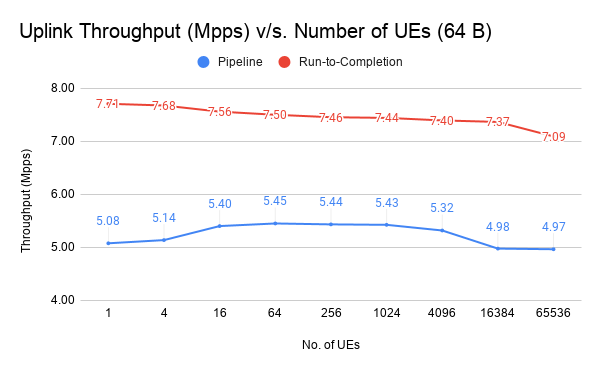
\includegraphics[width=70mm,height=50mm]{./fig/Results/tptv_snumues/UL.png}}
    \label{figULues}
    }
    \subfigure[]{
    \fbox{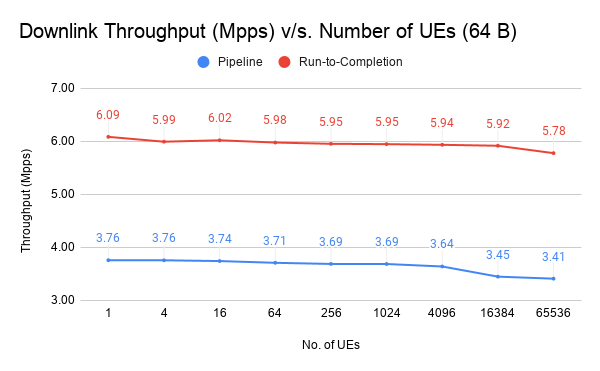
\includegraphics[width=70mm,height=50mm]{./fig/Results/tptv_snumues/DL.png}}
    \label{figDLues}
    }
    
    \caption{ Throughput (in Mpps) v/s number of active UEs. }
        \label{figureUEs}
\end{figure}

\subsubsection{Results}
There is slight/negligible degradation of performance for RTC model with the increasing number of sessions. Downlink throughput decreases for pipeline model with increase in number of sessions. No discernible pattern is observed for pipeline uplink. 

\subsection{Scaling of throughput with number of cores \label{subsectionThroughputScaling}}

The throughput is measured for 64 Byte payload and IMIX traffic (see \cite{imixLink}). The
 results are illustrated in Figure \ref{figure64Scaling} and Figure \ref{figureimixScaling}. The IMIX traffic models the standard internet traffic. The average payload size for IMIX distribution comes out to be 309 bytes. Each run is of the duration 150 seconds. The number of active sessions are 65536. The load generated at RAN/DNN exceeds the processing capacity of the UPF and the link is always saturated. The number of cores are varied across the runs to measure the total transmit throughput of the UPF in both uplink and downlink direction. 
 
RTC is expected to take fewer cores to saturate the transmit throughput than pipeline as per core throughput is higher for RTC (see section \ref{subSectiontptPayload}).
The number of cores required to saturate a given load in Gbps increases with decreasing payload size because the number of incoming packets increases with the decreasing payload size.
\begin{figure}[htbp]
    \centering
    \subfigure[]{
    \fbox{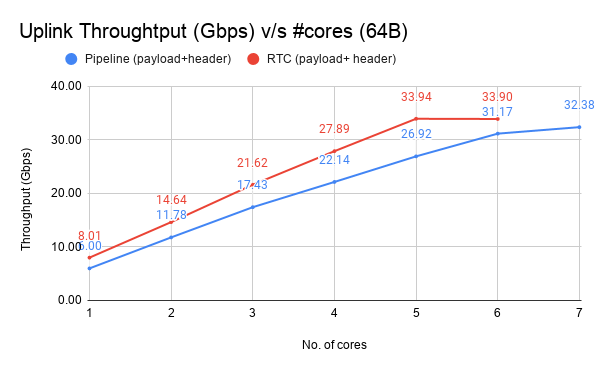
\includegraphics[width=70mm,height=50mm]{./fig/Results/64ByteThrouhgput/ULG.png}}
    \label{fig64ULG}
    }
    \subfigure[]{
    \fbox{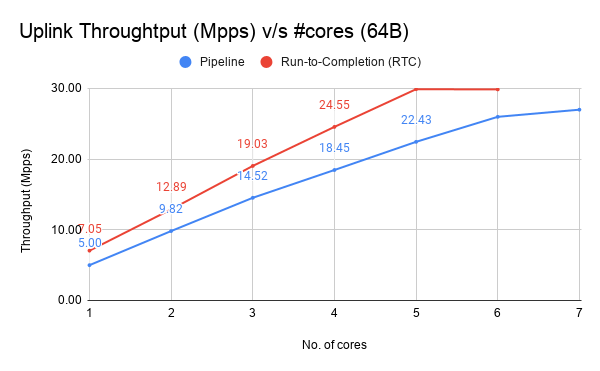
\includegraphics[width=70mm,height=50mm]{./fig/Results/64ByteThrouhgput/ULM.png}}
    \label{fig64ULM}
    }
    \subfigure[]{
    \fbox{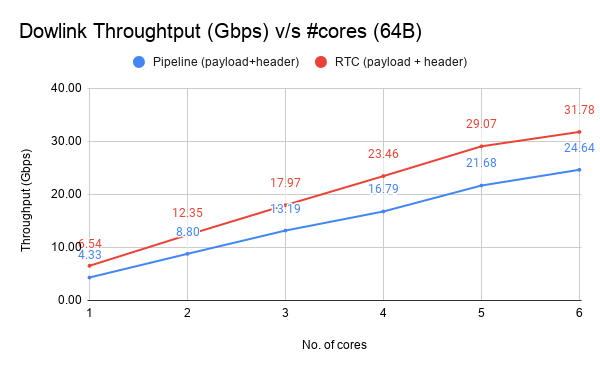
\includegraphics[width=70mm,height=50mm]{./fig/Results/64ByteThrouhgput/DLG.png}}
    \label{fig64DLG}
    }
    \subfigure[]{
    \fbox{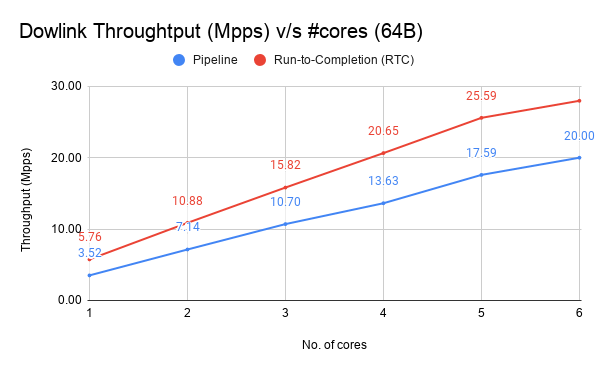
\includegraphics[width=71mm,height=50mm]{./fig/Results/64ByteThrouhgput/DLM.png}}
    \label{fig64DLM}
    }
    \caption{ Throughput v/s Number of Cores (64 Byte payload). Throughput calculation in Gbps includes header size.}
        \label{figure64Scaling}
    \end{figure}

\subsubsection{Results}
\begin{figure}[htbp]
    \centering
    \subfigure[]{
    \fbox{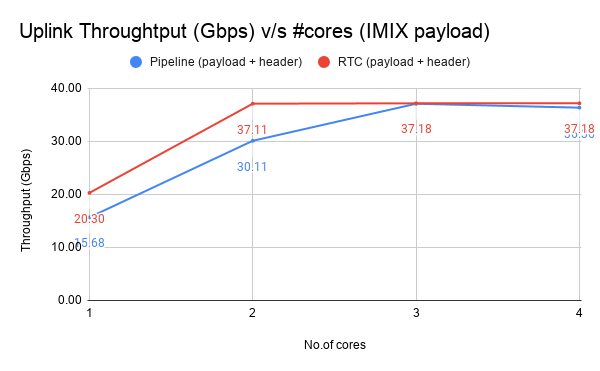
\includegraphics[width=70mm,height=50mm]{./fig/Results/imix/ULG.png}}
    \label{figimixULG}
    }
    \subfigure[]{
    \fbox{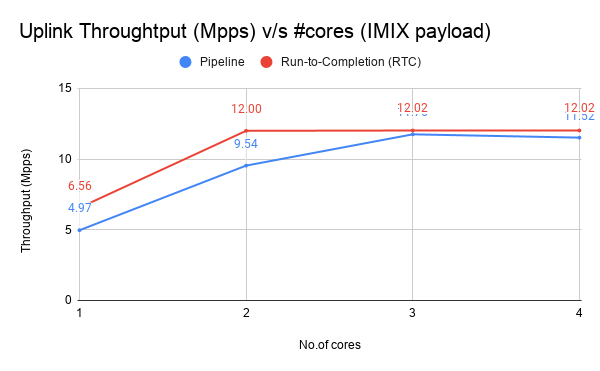
\includegraphics[width=70mm,height=50mm]{./fig/Results/imix/ULM.png}}
    \label{figimixULM}
    }
    \subfigure[]{
    \fbox{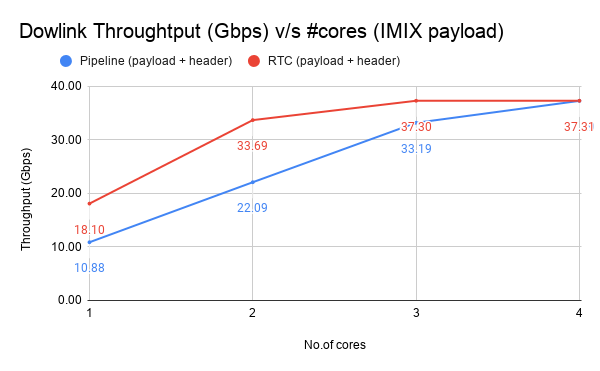
\includegraphics[width=70mm,height=50mm]{./fig/Results/imix/DLG.png}}
    \label{figimixDLG}
    }
    \subfigure[]{
    \fbox{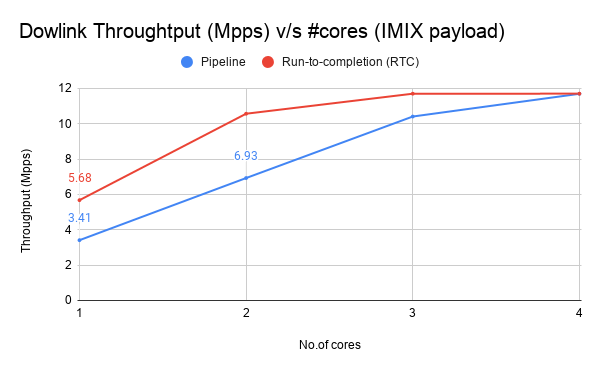
\includegraphics[width=70mm,height=50mm]{./fig/Results/imix/DLM.png}
    }
    \label{figimixDLM}
    }
    \caption{ Throughput v/s Number of cores (IMIX payload). Throughput calculation in Gbps includes header size.}
        \label{figureimixScaling}
    \end{figure}


\begin{itemize}
        \item For smaller sized packets (64 B in our case), the number of packets to be processed is quite large. Uplink RTC throughput is saturated in 5 cores. Uplink Pipeline is not saturated in even  6 cores. Downlink RTC throughput is saturated in 6 cores. Downlink Pipeline is not saturated.  
        \item For IMIX Uplink, RTC saturated in 2 cores. Pipeline saturated in 3 cores. For IMIX Downlink, RTC saturates in 3 cores. Pipeline saturates in 4 cores.
\end{itemize}
The difference in uplink and downlink perfomance is due to the GTP encapsulation overhead in the downlink direction.
\subsection{Handling Skewed Traffic \label{subsubsectionSkewedTraffic}}
The section \ref{RTCpipelineComparison} discusses the limitations of RTC model in handling skewed traffic. As the packets are redirected in hardware, RTC model has no flexibilty to redirect traffic from one core to another. 
The pipeline model can redistribute traffic (see Section \ref{secPipeline}).
\subsubsection{Experimental Setup}
The number of worker cores is kept fixed at 4 in both the models (excluding master core in pipeline model).
Initially a uniform  load is applied on all the worker cores. The load on a single UPF worker core is increased in steps while load on the remaining cores is kept fixed.
As RSS based packet redirection is random and uniform across cores, it is not possible to know apriori which session will be mapped to which core. Initially , packets were sent from 1024 different UE sessions and IP-Session ID to UPF core mapping was precomputed and stored
 in a file. This mapping was used to send packets on differential rate to the different UPF
  cores. For overloading a particular UPF core, the inter packet delay was reduced for the packets coming from RAN side. The rate limiting APIs were not available for the 40 Gbps NIC.
Sessions-IP were range partitioned for pipeline model. 
\begin{figure}[htbp]
    \centering
    \subfigure[]{
    \fbox{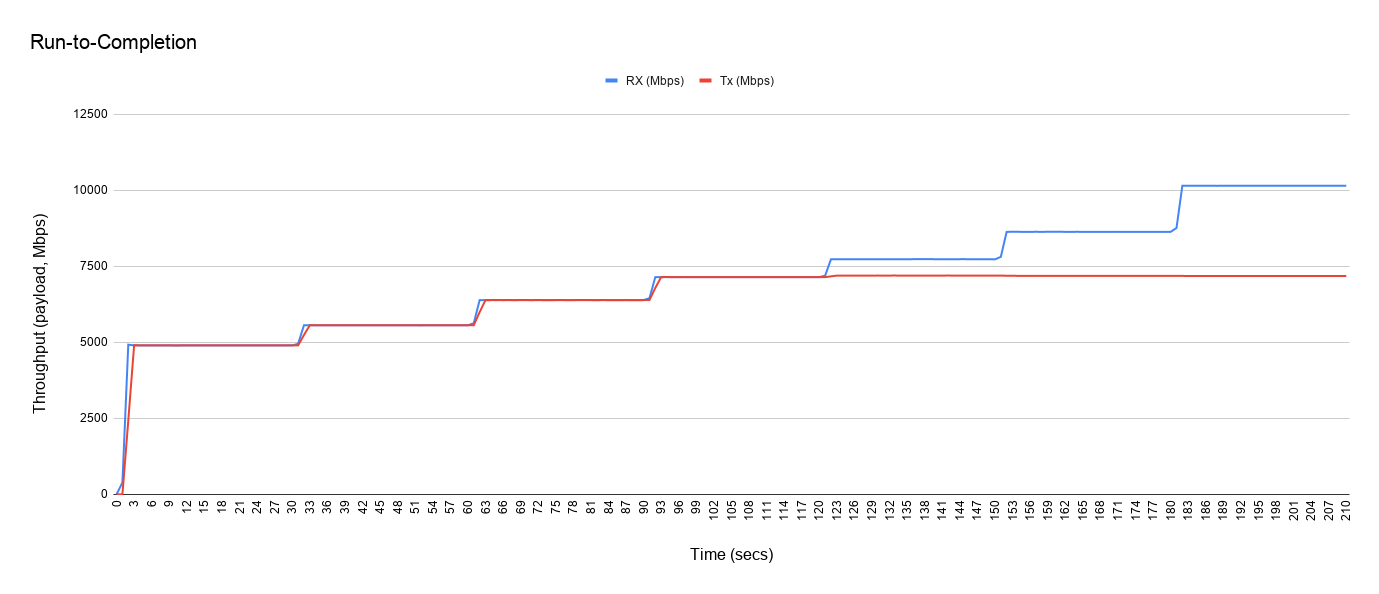
\includegraphics[width=\textwidth, keepaspectratio]{./fig/Results/UERedistribution/Run-to-Completion.png}}
    \label{figRTCskewed}
    }
    \subfigure[]{
    \fbox{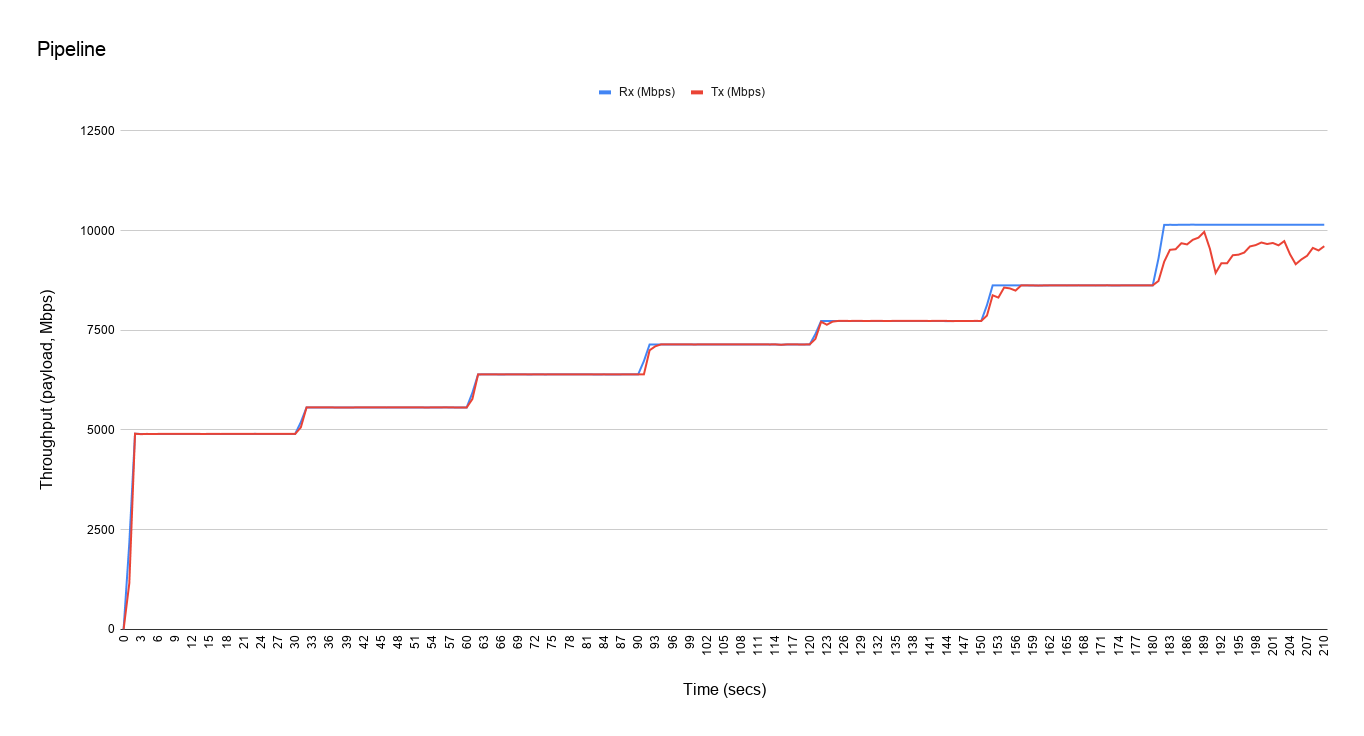
\includegraphics[width=\textwidth, keepaspectratio]{./fig/Results/UERedistribution/Pipeline.png}}
    \label{figPipelineSkewed}
    }
    \caption{ Handling of skewed UE traffic in pipeline and RTC models }
    \label{figureSkewed}
\end{figure}


\subsubsection{Results}
The results are illustrated in Figure \ref{figureSkewed}.
\begin{itemize}
    \item \textbf{RTC} Beyond the processing capability of a core, the increase in incoming traffic has no effect on the transmit throughput.The packets are dropped thereafter.
    \item \textbf{Pipeline} Pipeline handles the increasing load quite well by remapping
     some of the UEs to least loaded core. However,  it can be observed that pipeline
      Tx-throughput does not match the RX-throughput on the last step increase. This is because the total processing capability of all the worker cores is reached. 
\end{itemize}

\subsection{Dynamic Scaling \label{subsubsectionDynamicScaling}}
The section \ref{RTCpipelineComparison} discusses why dynamic scaling is a useful concept 
for energy efficiency and how pipeline may effectively handle dynamic reconfiguration with
 dropping of fewer packets and insignifcant impact on latency.

\subsubsection{Experimental Setup}
The maximum number of cores are kept at 4. Initially a single worker core is started (and
one master core for pipeline). The payload size is kept at 64 Bytes. The experiment is run
for 300 seconds. The load is increased in step size of 5 Gbps (payload + header) every 60 
seconds.
The overload detection algorithm for different models is 
\begin{itemize}
    \item  \textbf{RTC} The idea of exponential weighted moving average (EWMA) (see \cite{ewma})
     was used for calculating core load factor. When the core load factor reaches above a
      threshold, port is stopped, hardware queues and RSS hash is reconfigured, the port
       is restarted and a new core is launched for forwarding of packets.
    The core load factor is calculated after every polling event. 
   \[ averageCLF = 0.999 * averageCLF + 0.0001 * (number of packets Received)/32\] 
   A maximum of 32 packets can be received on every polling event. $0.001$ is the weight 
   assigned to the current load factor. EWMA is resilient to transient overload and is influenced by both the current and previous value of the load factor.

    \item \textbf{Pipeline} The EWMA technique was not feasible for Pipeline model. 
        The software rings were used for communication between master and worker cores. A function call was required for calculating the existing number of elements in the ring. The performance is degraded substantially if this function is called after every polling event on master core. As a workaround, core load factor was sampled every millionth packet. If the core overload is detected for a certain number of consecutive time, the core is deemed to be overloaded and a new core is launched.
\end{itemize}

\subsubsection{Results}
The results are illustrated in Figures \ref{figuredynamicScaling1} and \ref{figuredynamicScaling2}.
\begin{itemize}
    \item \textbf{RTC}: Figure \ref{figdynamicRTC1} shows the entire run of the experiments for pipeline model. The spike in latency  and sharp drop in throughput is observed whenever a new core is launched (see Figure \ref{figdynamicRTC2}). The maximum latency observed during the reconfiguration is around 100 ms. The reconfiguration time is around 400 ms. 
    \item \textbf{Pipeline}: Figure \ref{figdynamicPipeline1} shows the entire run of the experiments.  No appreciable change  is observed in throughput  or latency (see Figure \ref{figdynamicPipeline2}). The reconfiguration time is around 130 us. 
\end{itemize}
\begin{figure}[htbp]
    \centering
    \subfigure[]{
    \fbox{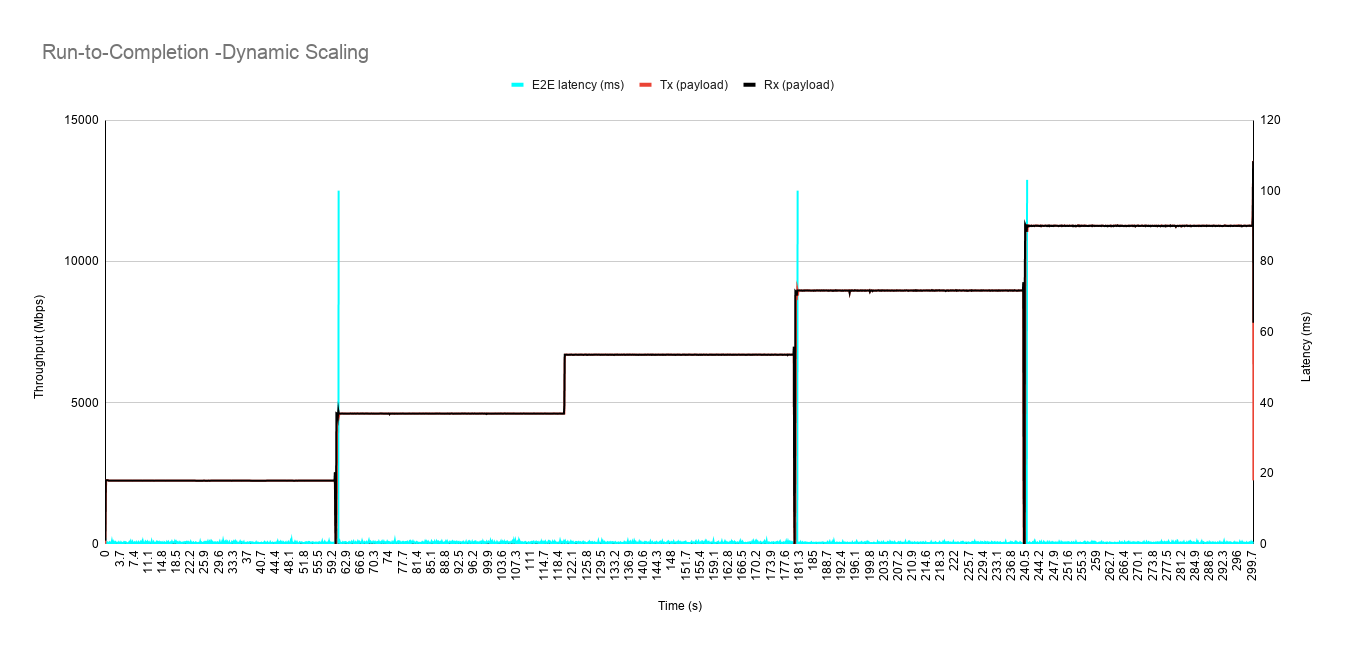
\includegraphics[width=\textwidth, keepaspectratio]{./fig/Results/dynamicScaling/RTC1.png}}
    \label{figdynamicRTC1}
    }
    \subfigure[]{
    \fbox{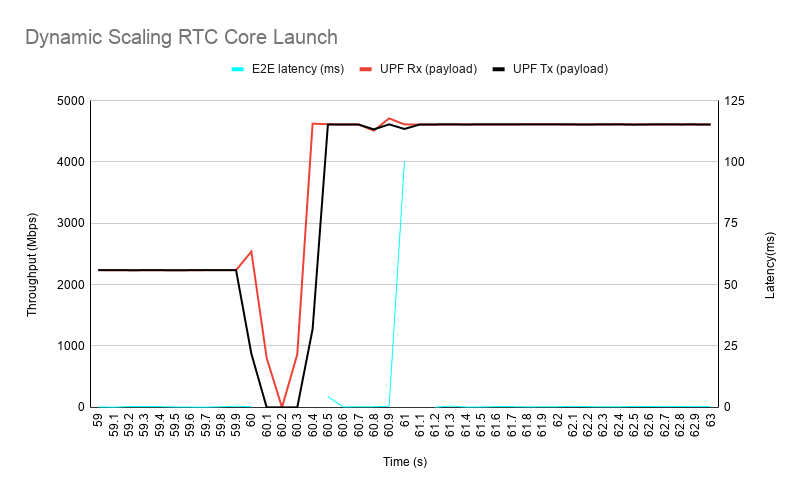
\includegraphics[width=\textwidth, keepaspectratio]{./fig/Results/dynamicScaling/RTC2.png}}
    \label{figdynamicRTC2}
    }
    \caption{RTC: Figure \subref{figdynamicRTC1}  shows throughput and end to end latency during the whole run. Figure \subref{figdynamicRTC2} shows the output during one of the core launches (the first one). }
    \label{figuredynamicScaling1}
\end{figure}
\begin{figure}[htbp]
    \centering
    \subfigure[]{
    \fbox{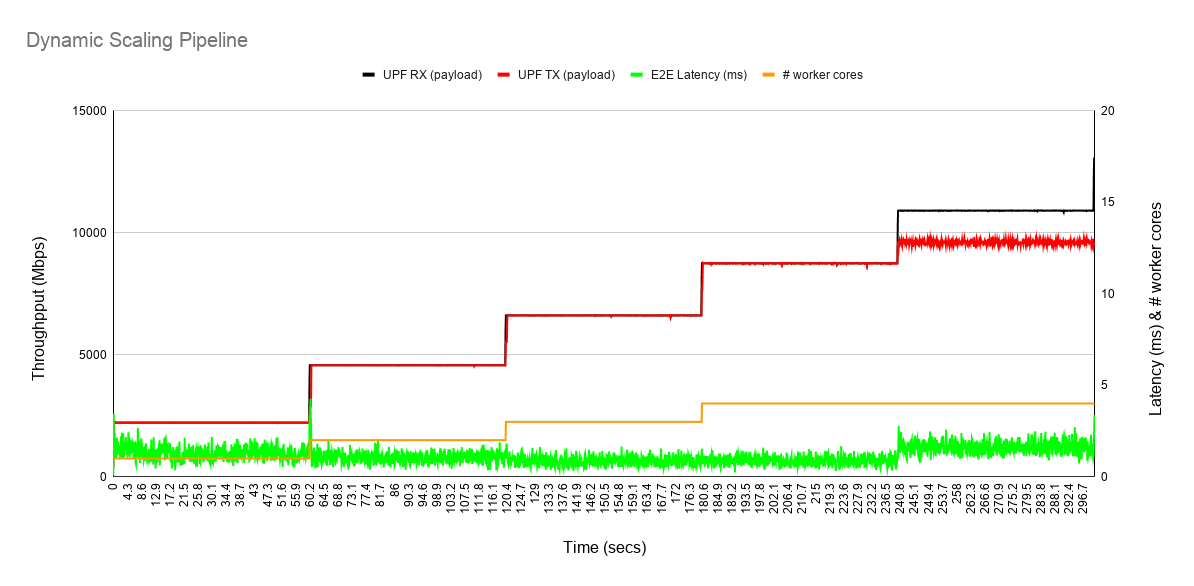
\includegraphics[width=\textwidth, keepaspectratio]{./fig/Results/dynamicScaling/Pipeline1.png}}
    \label{figdynamicPipeline1}
    }
    \subfigure[]{
    \fbox{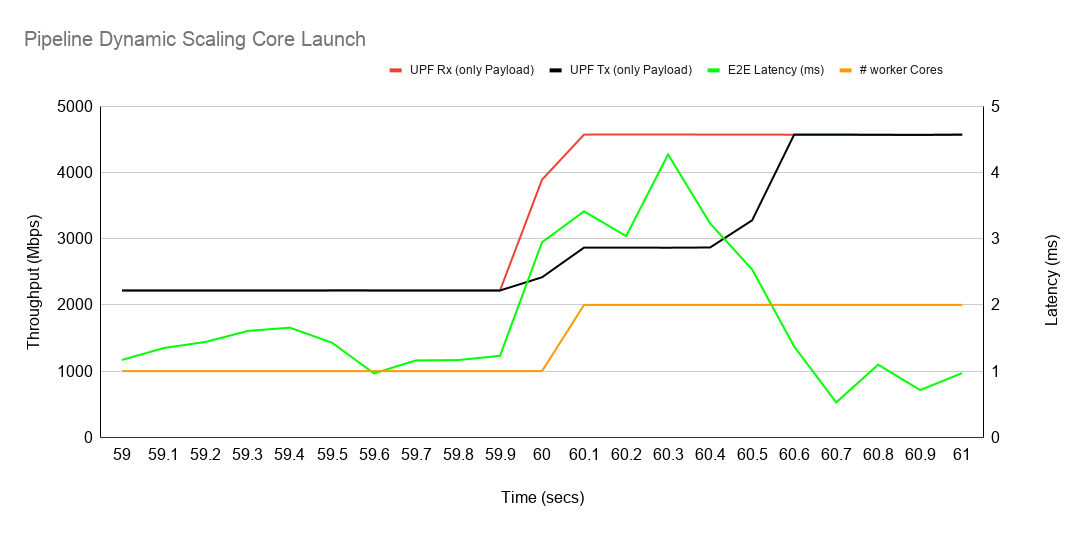
\includegraphics[width=\textwidth, keepaspectratio]{./fig/Results/dynamicScaling/Pipeline2.png}}
    \label{figdynamicPipeline2}
    }
    \caption{Pipeline: Figure \subref{figdynamicPipeline1} shows throughput and end to end latency during the whole run. Figure \subref{figdynamicPipeline2} shows the output during one of the core launches (the first one). }
        \label{figuredynamicScaling2}
\end{figure}

\section{Summary \label{secSummaryResults}}
The main question explored in these experiments was to define and evaluate different scenarios in which one model of execution is better than the other among the Pipeline and RTC models (also see section \ref{RTCpipelineComparison}). The effect of  the number of cores and the increase  in the number of  active sessions on throughput was also observed.
The important findings are 
\begin{itemize}
    \item RTC gives better per core throughput (30-40\% higher) than Pipeline.
    \item Throughput scales linearly with the number of cores. RTC gets saturated earlier because of higher per core throughpu Throughput scales linearly with the number of cores. RTC gets saturated earlier because of higher per core throughput. 
    \item The average throughput was not affected significantly by the increase in number of sessions.
    \item Pipeline model can handle skewed traffic effectively by redistribution of the traffic. 
    \item The number of packets dropped and  the impact on latency is quite low  for pipeline model while dynamically increasing the number of cores to handle the higher incoming traffic.

\end{itemize}